\documentclass[10pt,a4paper]{article}
\usepackage[utf8]{inputenc}
\usepackage[french]{babel}
\usepackage[T1]{fontenc}
\usepackage{amsmath}
\usepackage{amsfonts}
\usepackage{amssymb}
\usepackage{graphicx}
\usepackage[left=2cm,right=2cm,top=2cm,bottom=2cm]{geometry}

\title{Diffraction of light by any opening}
\author{PLASSE Jonathan, ROUSSEL Loïc, ROHR Julien, NAÏLI Kamel}

\begin{document}
\maketitle

\section{History of Diffraction}
The diffraction is a phenomenon discovered in 1665 by Francesco Maria Grimaldi. Locked into a dark room, this physicist, showing interest in optics and astronomy, enjoied drilling tiny openings in an black curtain exposed to the sun. He used these sources of improvised light and interposed on the path of the beam either slots of different shape or hair or even feathers of birds. Every time, he observed on a screen placed behind these objects, iridescent fringes located apart from the normal geometrical route. He makes then the assumption that the change of trajectory of the light infered by the presence of an hurdle or an openings, is the consequence of a new phenomenon, namely the diffraction. He announces this discovery in his paper " Physico-mathesis of Lumine, coloribus and iride ".

Christian Huygens ( 1629-1695 ) was also interested in this new phenomenon. In 1678, he writes a short paper " Treatedwith the light " and layed the foundations for the undulatory theory of the light. By analogy with the distribution of the waves on the surface of the water or the sound waves in the air, he assumed that the light propagated under the spherical shape of waves, and that every point reached by the wave behaved as a new secondary source. However his analogy went too far since to his mind, the bright vibration was longitudinal and needed a material middle to propagate. Incapable to define exactly the nature of this middle, he called it " the ether ". 

The theory of ondelettes allowed him to find for instance the laws of the refraction of Snell-Descartes. This theory was complimented by Newton ( 1642-1727 ) who also observed the phenomena of diffraction and the localized fringes infered by thin blades and developed a corpuscular theory. 

After the highlighting of interference fringes by his famous double slots, Thomas Young (1773-1829) relaunched the undulatory theory of the light. Augustin Fresnel (1788-1827) generalized the approach of Huygens and imagined two new devices to obtain interferences: mirrors and biprisme of Fresnel. The principle of Huygens Fresnel allows by the integral calculus to find accurately the diffraction patterns whatever the shape of the slot are. 

Fraunhofer discovered in 1814 the rays of discontinuity in the solar spectrum: what allowed him to invent the spectroscope one year later. Besides, he was the first one to study the diffraction of the light with optical networks (networks of Fraunhofer) which he used to measure accurately the optical properties of glasses (refractive index). 

The equations of James-Clerk Maxwell (1831-1879) on electromagnetism support the wave theory of light. We will have to wait for Albert Einstein in 1905 with the emergence of quantum physics to reestablish a corpuscular aspect and bring these two theories together.

\section{The diffraction regimes}
	\subsection{Fresnel diffraction}
Fresnel diffraction or near field diffraction is a near field description of the physical diffraction phenomenon. It takes into account the curvature of the wavefront, and therefore the variation of the phase term resulting from the propagation in the spherical shape of the light in accordance with the principle of Huygens Fresnel. For each point of the space and considered independent, the reception of a wave of amplitude E (M, t) , triggers the repetition of a spherical wave of the same frequency, same amplitude and same phase. Instead of considering that the wave progresses continuously, its progression is decomposed by imagining that it is progressing step by step. The diffraction pattern arising from any slot will be an integration calculation. 

The equation of propagation of a spherical wave is:

\[E(r,t)= \frac{E_0}{r} e^{j(kr-\omega t)}\]

The elementary variation of E (r, t) by the principle of Huygens Fresnel:

\[dE=\frac{e^{jkr}}{r} E(x',y') dx' dy'\]

By the use of the Helmoltz equation in a homogeneous medium: 

\[\Delta E+k^2 E=0\]

And by integration on the surface of the opening of the slot, we obtain:

\[E(x,y)=\frac{1}{j\lambda} \iint \frac{e^{jkr}}{r}E(x',y')dx'dy'\]

	\subsection{The diffraction of Fraunhofer}
The Fraunhofer diffraction is an approximation in far-field, namely observation at great distance. The radius of curvature of the diffracted waves is therefore very large, so that they can be considered as plane waves. This approximation can also be done when one wants the diffraction pattern in the image focal plane of a converging lens. The advantage is that it allows us to go through a Fourier transform calculation already implemented in a python library.

\begin{center}
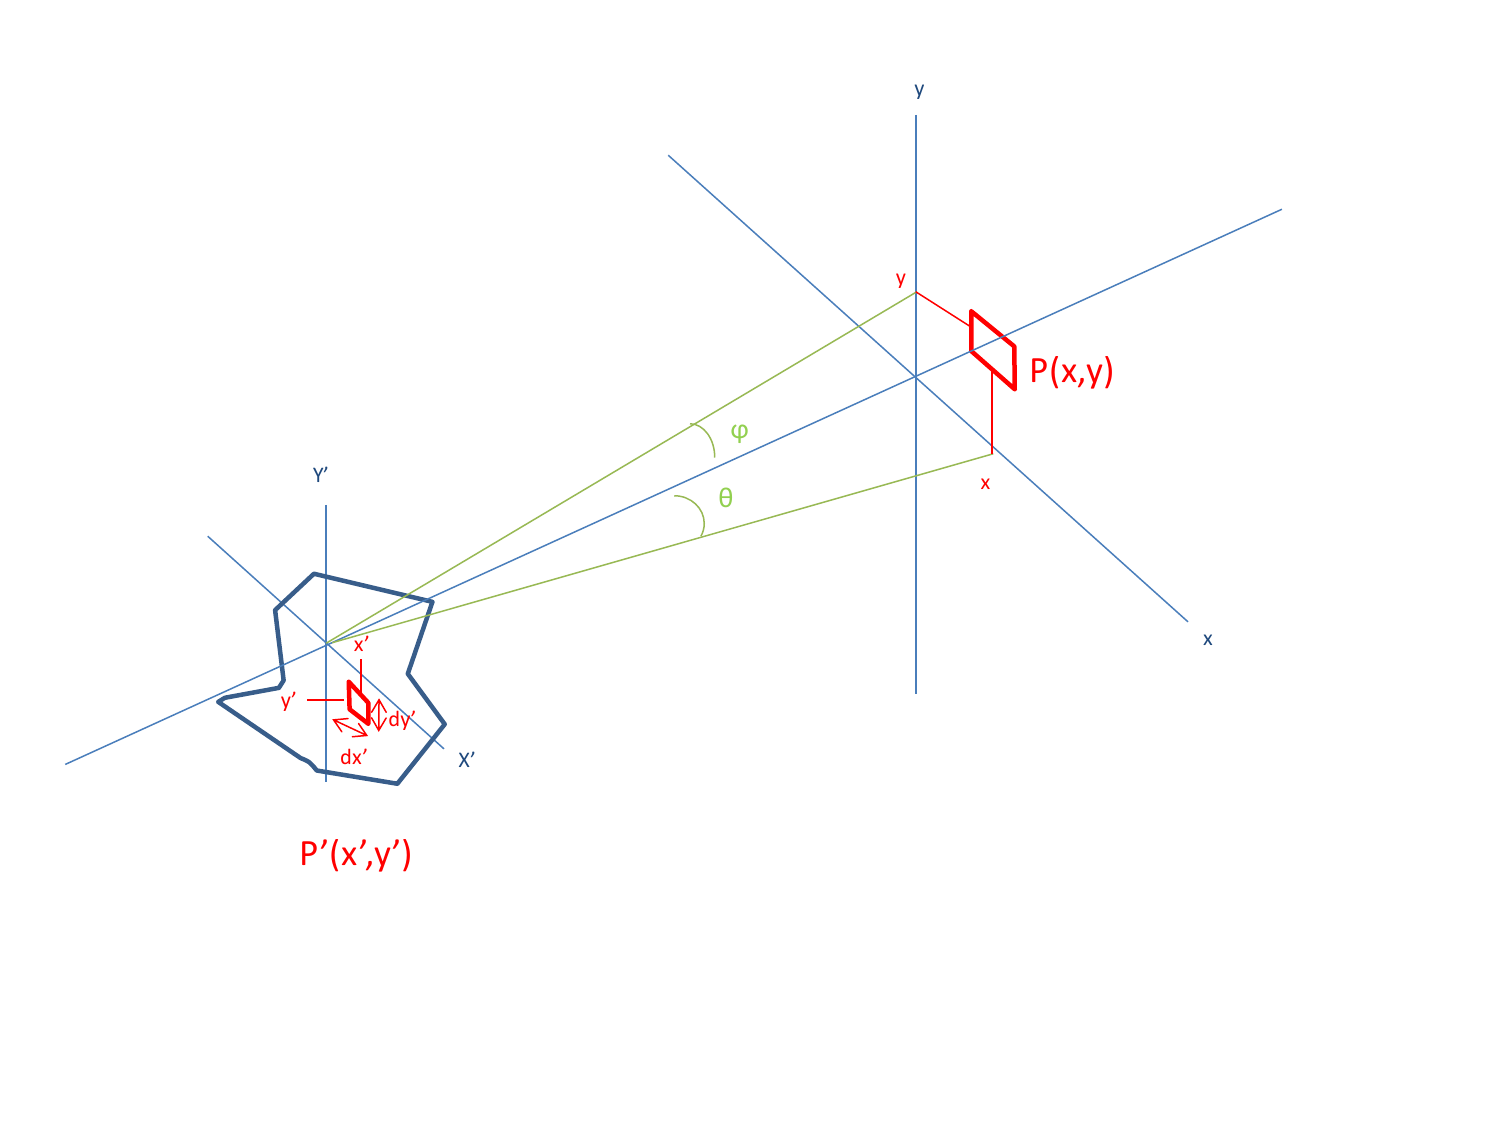
\includegraphics[scale=0.32]{../Ressources/schema-1.png}
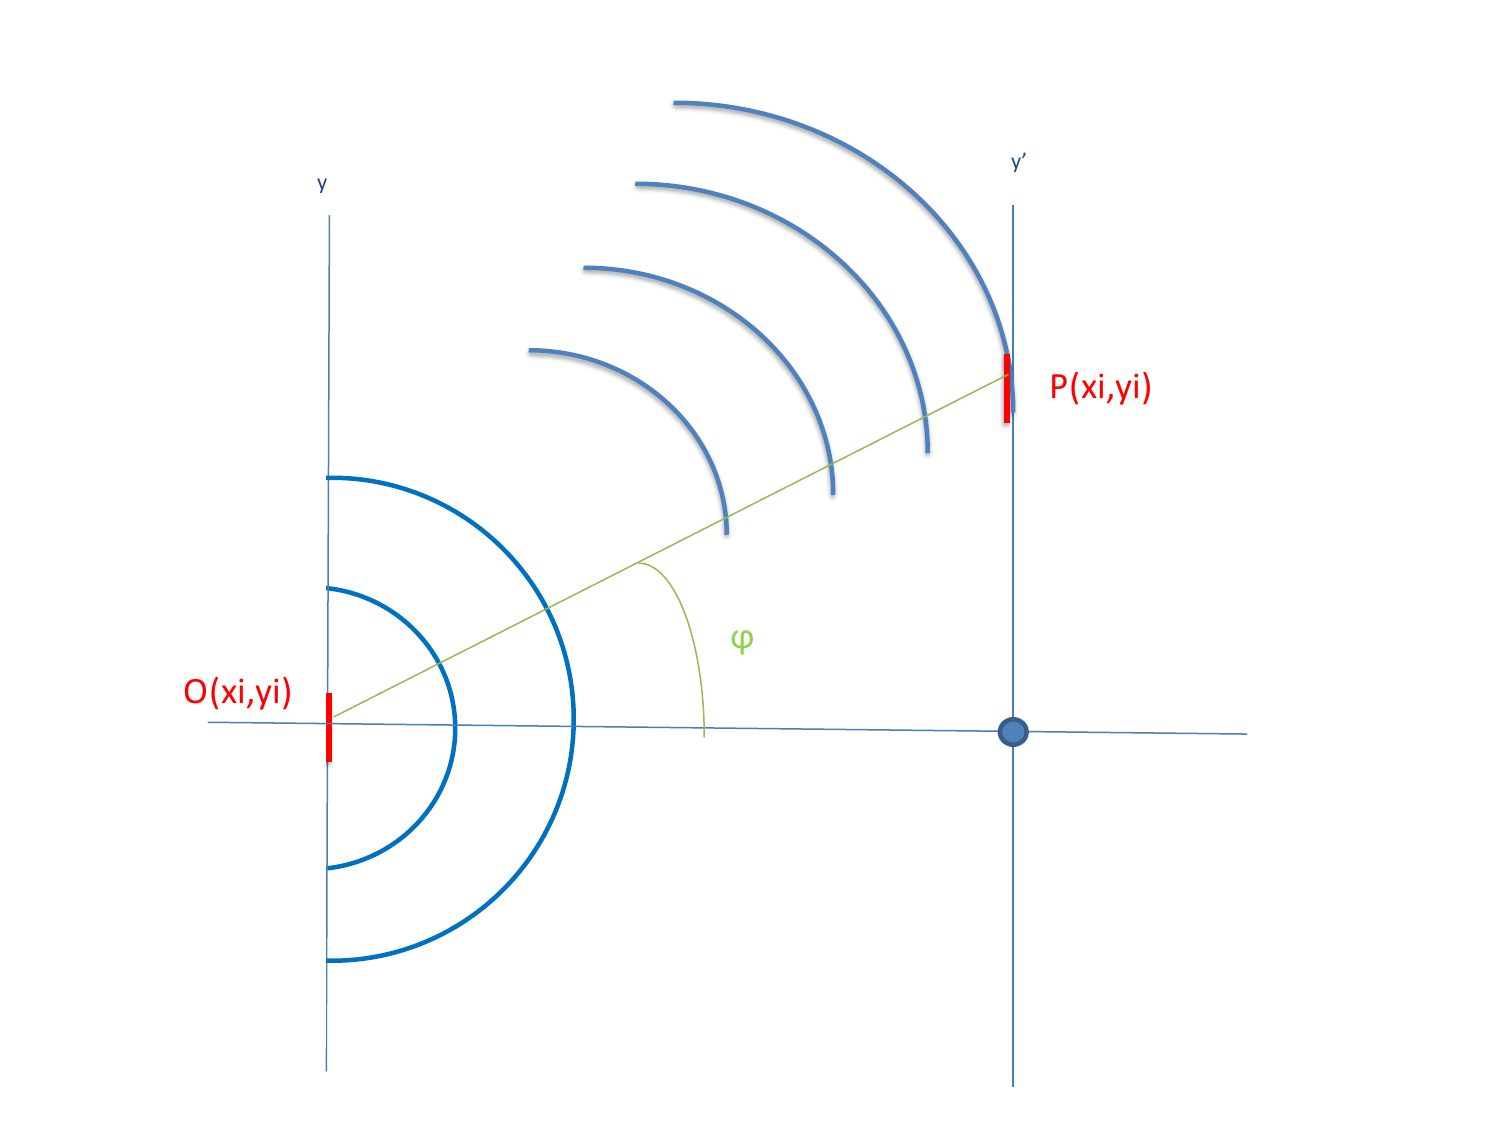
\includegraphics[scale=0.32]{../Ressources/schema-2.png}
\end{center}

\[r=\sqrt{z^2+(x-x')^2+(y-y')^2}\]
\[r=z\sqrt{1+\frac{(x-x')}{z_i}^2+\frac{(y-y')}{z_i}^2}\]

In Fraunhofer’s regime:

\[z^2\gg(x-x')^2+(y-y')^2\]

We can carry out a development limited to order 1: 

\[r=z\left(1+\frac{(x-x')}{2z_i}^2+\frac{(y-y')}{2z_i}^2\right)\]

After development:

\[r \approx z+\frac{x^2+y^2}{2z}+\frac{x'^2+y'^2}{2z}-\frac{xx'+yy'}{z}\]

Approximation valid in the Fresnel region. 

If we are very far from the source, the last term becomes negligible and we find ourselves in the Fraunhofer region.

\begin{center}
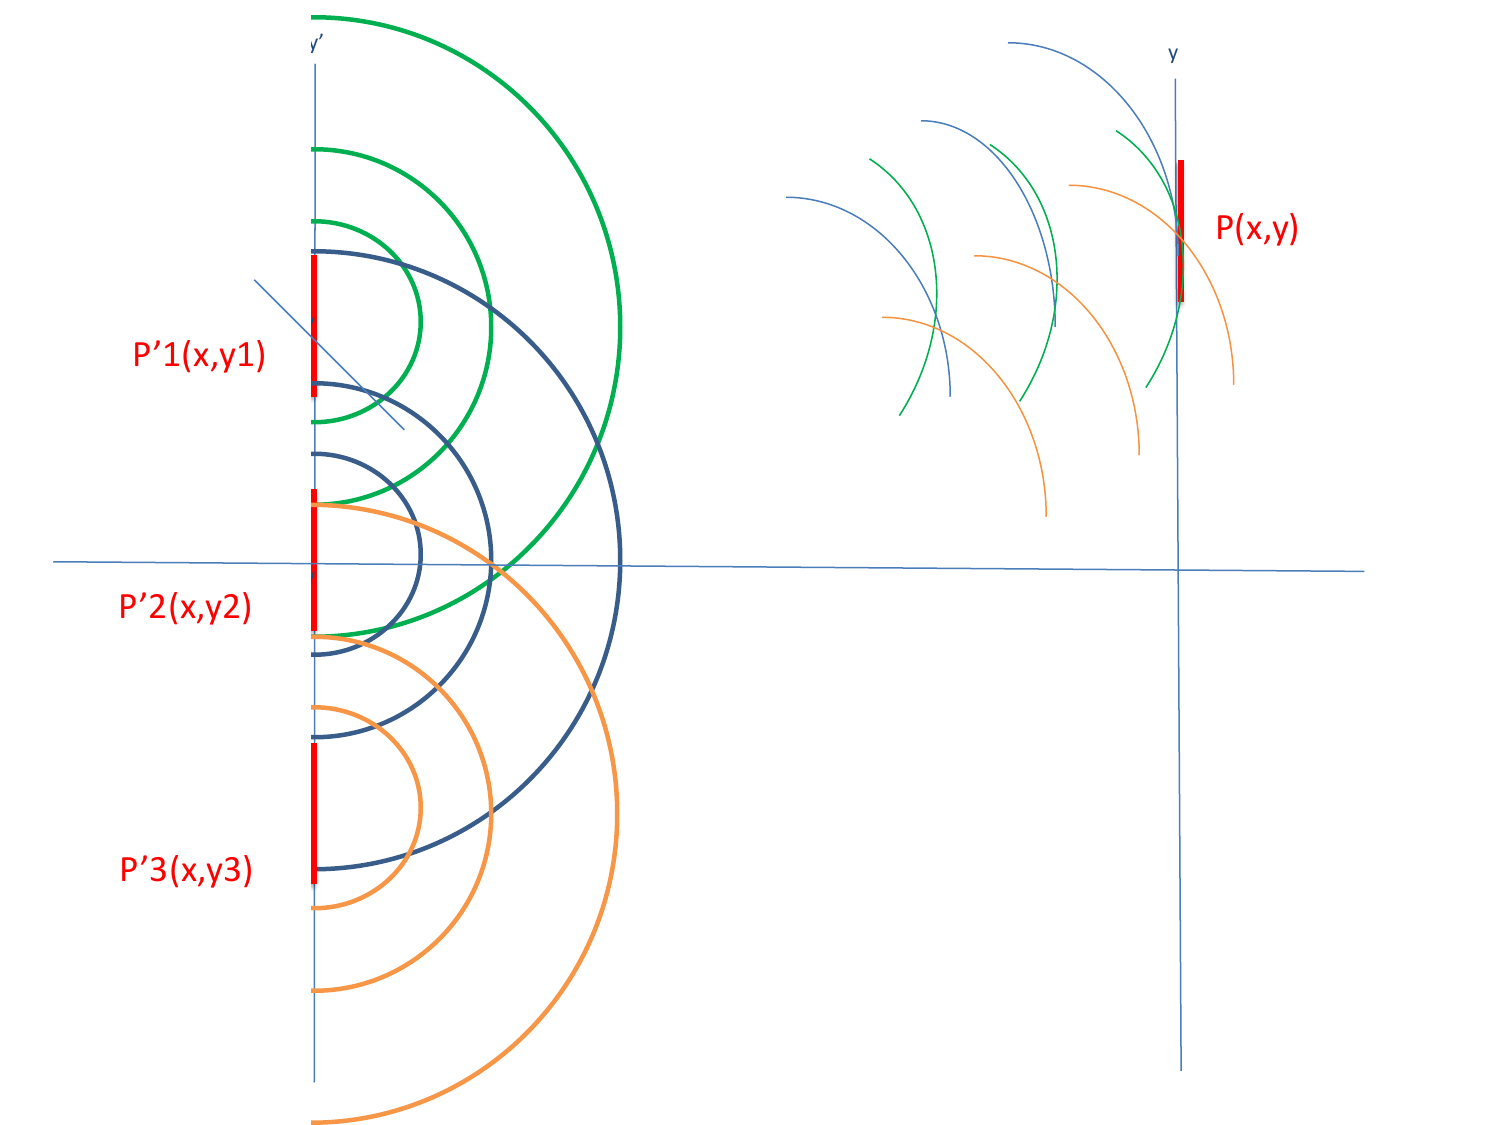
\includegraphics[scale=0.32]{../Ressources/schema-3.png}
\end{center}

\[r \approx z+\frac{x^2+y^2}{2z}-\frac{xx'+yy'}{z}\]

\[E(x,y)=\frac{1}{j\lambda} \iint \frac{e^{jkr}}{r}E(x',y')dx'dy'\]

With $r\approx z$ at the denominator for the damping term of the wave and $r \approx z+\frac{x^2+y^2}{2z}-\frac{xx'+yy'}{z}$ for the term of phase:

\[E(x,y)=\frac{1}{j\lambda z} e^{jk\left(z+\frac{x^2+y^2}{2z}\right)}\iint e^{-jk\frac{xx'+yy'}{z}}E(x',y')dx'dy'\]

Let $f_x=\frac{x}{\lambda z}$ and $f_x=\frac{y}{\lambda z}$

\[E(x,y)=\frac{1}{j\lambda z} e^{jk\left(z+\frac{x^2+y^2}{2z}\right)}\underbrace{\iint e^{-2\pi j(f_xx'+f_yy')}E(x',y')dx'dy'}_\text{Fourier's transformation}\]

Polar coordinates in the Fraunhofer regime:

\[x=\rho \cos(\omega) \]
\[y=\rho \sin(\omega) \]
\[x'=\rho \cos(\omega') \]
\[y'=\rho \sin(\omega') \]

Elementary area: $dxdy=\rho d\rho d\omega$

So, we use the expression Cartesian:

\[E(\rho,\omega)=\frac{1}{j\lambda z} e^{jk\left(z+\frac{\rho^2 \cos(\omega)^2+\rho^2 \sin(\omega)^2}{2z}\right)}\iint e^{-jk\frac{\rho \cos(\omega)\rho' \cos(\omega')+\rho \sin(\omega)\rho' \sin(\omega)'}{z}}E(\rho',\omega')\rho' d\rho'd\omega'\]

\[E(\rho,\omega)=\frac{1}{j\lambda z} e^{jk\left(z+\frac{\rho^2}{2z}\right)}\iint e^{-jk\frac{\rho\rho'\cos(\omega-\omega')}{z}}E(\rho',\omega')\rho' d\rho'd\omega'\]

\end{document}